\documentclass[tikz]{standalone}

\begin{document}
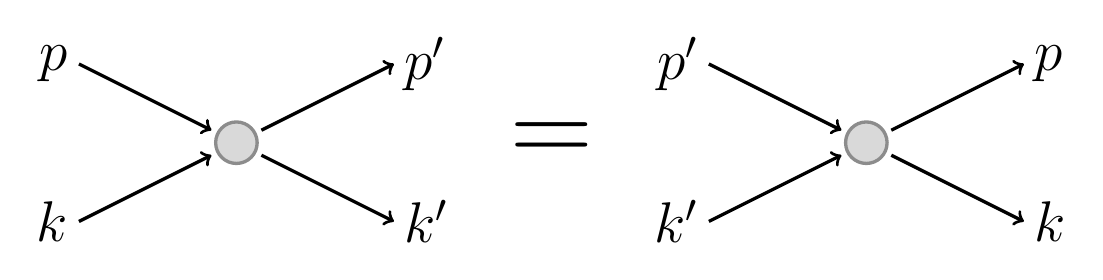
\begin{tikzpicture}[
    very thick,font=\huge,
    col/.style={circle,draw=gray!90,fill=gray!30,minimum size=15},
    incom/.style={<-,shorten <=2},
    outgo/.style={->,shorten <=2}
  ]

  \node[scale=2] (eq) at (0,0) {=};
  \coordinate[col] (col1) at eq++(-4,0);
  \coordinate[col] (col2) at eq++(4,0);

  \draw[outgo] (col1) -- ++(2,1) node[right] {$p^\prime$};
  \draw[outgo] (col1) -- ++(2,-1) node[right] {$k^\prime$};
  \draw[incom] (col1) -- ++(-2,1) node[left] {$p$};
  \draw[incom] (col1) -- ++(-2,-1) node[left] {$k$};

  \draw[outgo] (col2) -- ++(2,1) node[right] {$p$};
  \draw[outgo] (col2) -- ++(2,-1) node[right] {$k$};
  \draw[incom] (col2) -- ++(-2,1) node[left] {$p^\prime$};
  \draw[incom] (col2) -- ++(-2,-1) node[left] {$k^\prime$};

\end{tikzpicture}
\end{document}
